\section{Design}
I dette projekt er der valgt så vidt muligt at designe alle løsninger med analog elektronik. Derfor er det valgt at forforstærkeren bygges af commonemittertrin med uafkoblet emittermodstand. Et commonemittertrins generelle opbygning er vist på figur \ref{fig:cekobling}.

\begin{figure}[h]
\centering
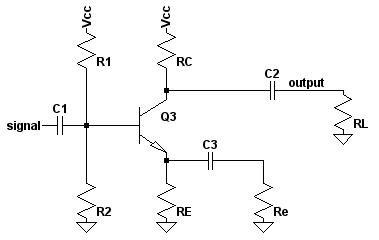
\includegraphics[scale=.6]{teknisk/forforstaerker/ceopkobling.png}
\caption{Generel form på commonemitterkobling med uafkoblet emittermodstand}
\label{fig:cekobling}
\end{figure}


Argumentet for dette valg er at det er det eneste trin, blandt commonemitter, -base og -collector, hvis spændingsforstærkning ikke afhænger af transistorparametre. Da transistorparametre blandt andet er afhængige af den anvendte transistors temperatur er det en betragtelig styrke ikke at skulle tage højde for dem. Spændingsforstærkningen i commonemittertrinnet er dog kun uafhængig af transistorparametre så længe følgende er gældende: $r_o >>R_C \| R_L$ og $i_e \approx i_c$.
Disse antagelser vil være gældende gennem hele designet af forforstærkeren. 
Forforstærkeren bygges af to commonemittertrin for at opnå den ønskede forstærkning på 63,3 gange. Dette skyldes at forstærkningen er givet ved ligning \ref{eq:gmbevis}.

\begin{equation}
A_v =  \frac{-gm \cdot R'_L}{1+gm \cdot R'_e} \approx  -\frac{R'_L}{R'_e} \Biggr\vert _{\frac{1}{gm}<R'_e}
\label{eq:gmbevis}
\end{equation}

Hvor $R'_e = R_e || R_E$ og $R'_L = R_L||R_C$. Det vil sige at jo tættere $R_e$ kommer på $\frac{1}{gm}$ jo mere indflydelse vil denne have på forstærkningen.

Det første trin skal have en forstærkning på 10 gange og det andet på 6,33 for at opnå den ønskede forstærkning, som vist på figur \ref{blok_forforstaerker}.

\begin{figure}[h]
\centering
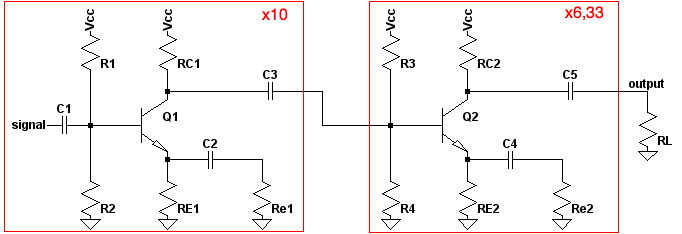
\includegraphics[scale=.6]{teknisk/forforstaerker/blok_forforstaerker.png}
\caption{Blokdiagram over forforstærkerens byggeblokke samt lydsignalets vej}
\label{blok_forforstaerker}
\end{figure}

For at opnå så lav forvrængning som muligt designes hvert trin således at DC-forstærkningen er så stor som muligt for at have meget at tilbagekoble. At AC- og DC-forstærkningen kan være forskellige muliggøres af den AC-koblede $R_e$, da denne kun vil have indflydelse på AC-forstærkningen.

\subsection*{Design af trin et}
Begge trin designes efter maksimal DC-forstærkning, som er givet ved ligning \ref{eq:dcgain}.

\begin{equation}
|A_{v}|=\frac{1}{\left(\frac{V_t \cdot R_C}{V_{R_C}}+\frac{R'_S}{\beta}\right) \left(\frac{1}{R_C}+\frac{1}{R_L}\right)}
\label{eq:dcgain}
\end{equation}
Hvor $R'_S = R'_S||R_1||R_2$ og $V_t = 26 \cdot 10^{-3}$.

For at designe et kredsløb med maksimal DC-forstærkning justeres størrelsen af $R_C$ uden at variere spændingen over den, $V_{R_C}$. Den maksimale $R_C$ findes ved ligning \ref{eq:rcmaks}.

\begin{equation}
R_{C,maks} = 
\end{equation}

Det første forstærkertrin skal tillade et spændingsudsving på udgangen, som er en faktor 10 større end mikrofonens peak outputspænding altså 316 mV. 


\subsection*{Design af trin to}



